\begin{figure}[h]
    \centering
    \begin{subfigure}[b]{0.3\textwidth}
        \centering
        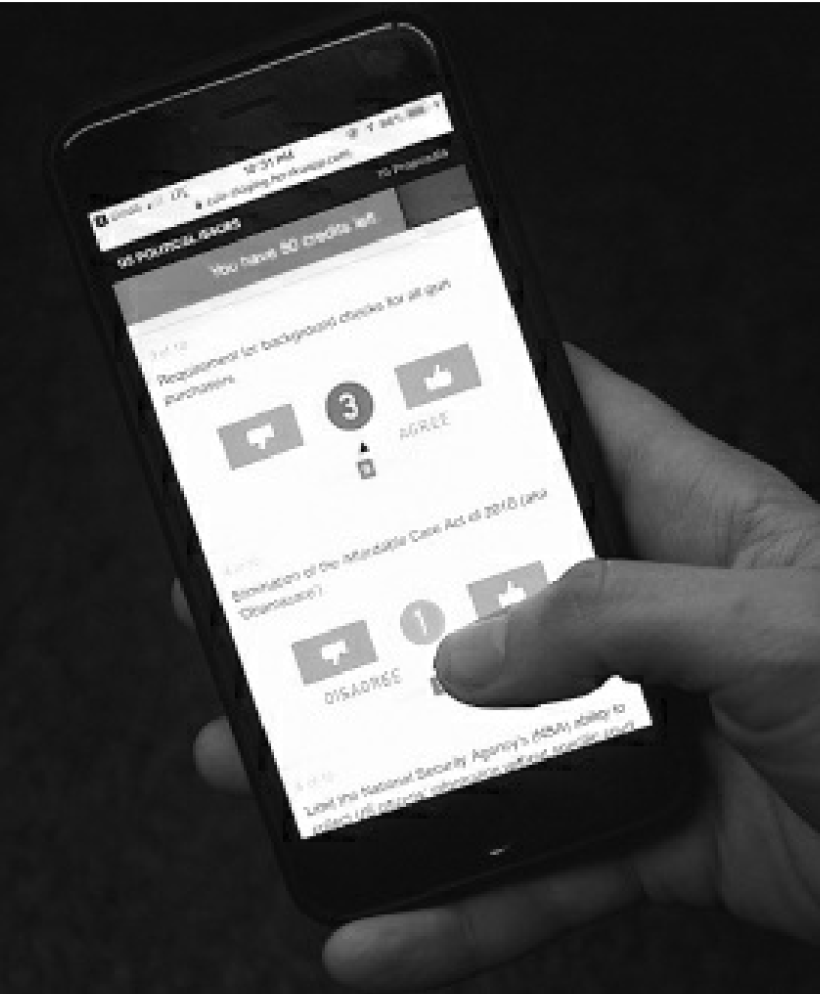
\includegraphics[width=\textwidth]{content/image/curr_interface/radical_market_wedesign.png}
        \caption{Software designed by WeDesign used in~\cite{quarfoot2017quadratic}. Image taken from~\cite{posner2018radical}.}
        \label{fig:wedesignInterface}
    \end{subfigure}
    \hfill
    \begin{subfigure}[b]{0.3\textwidth}
        \centering
        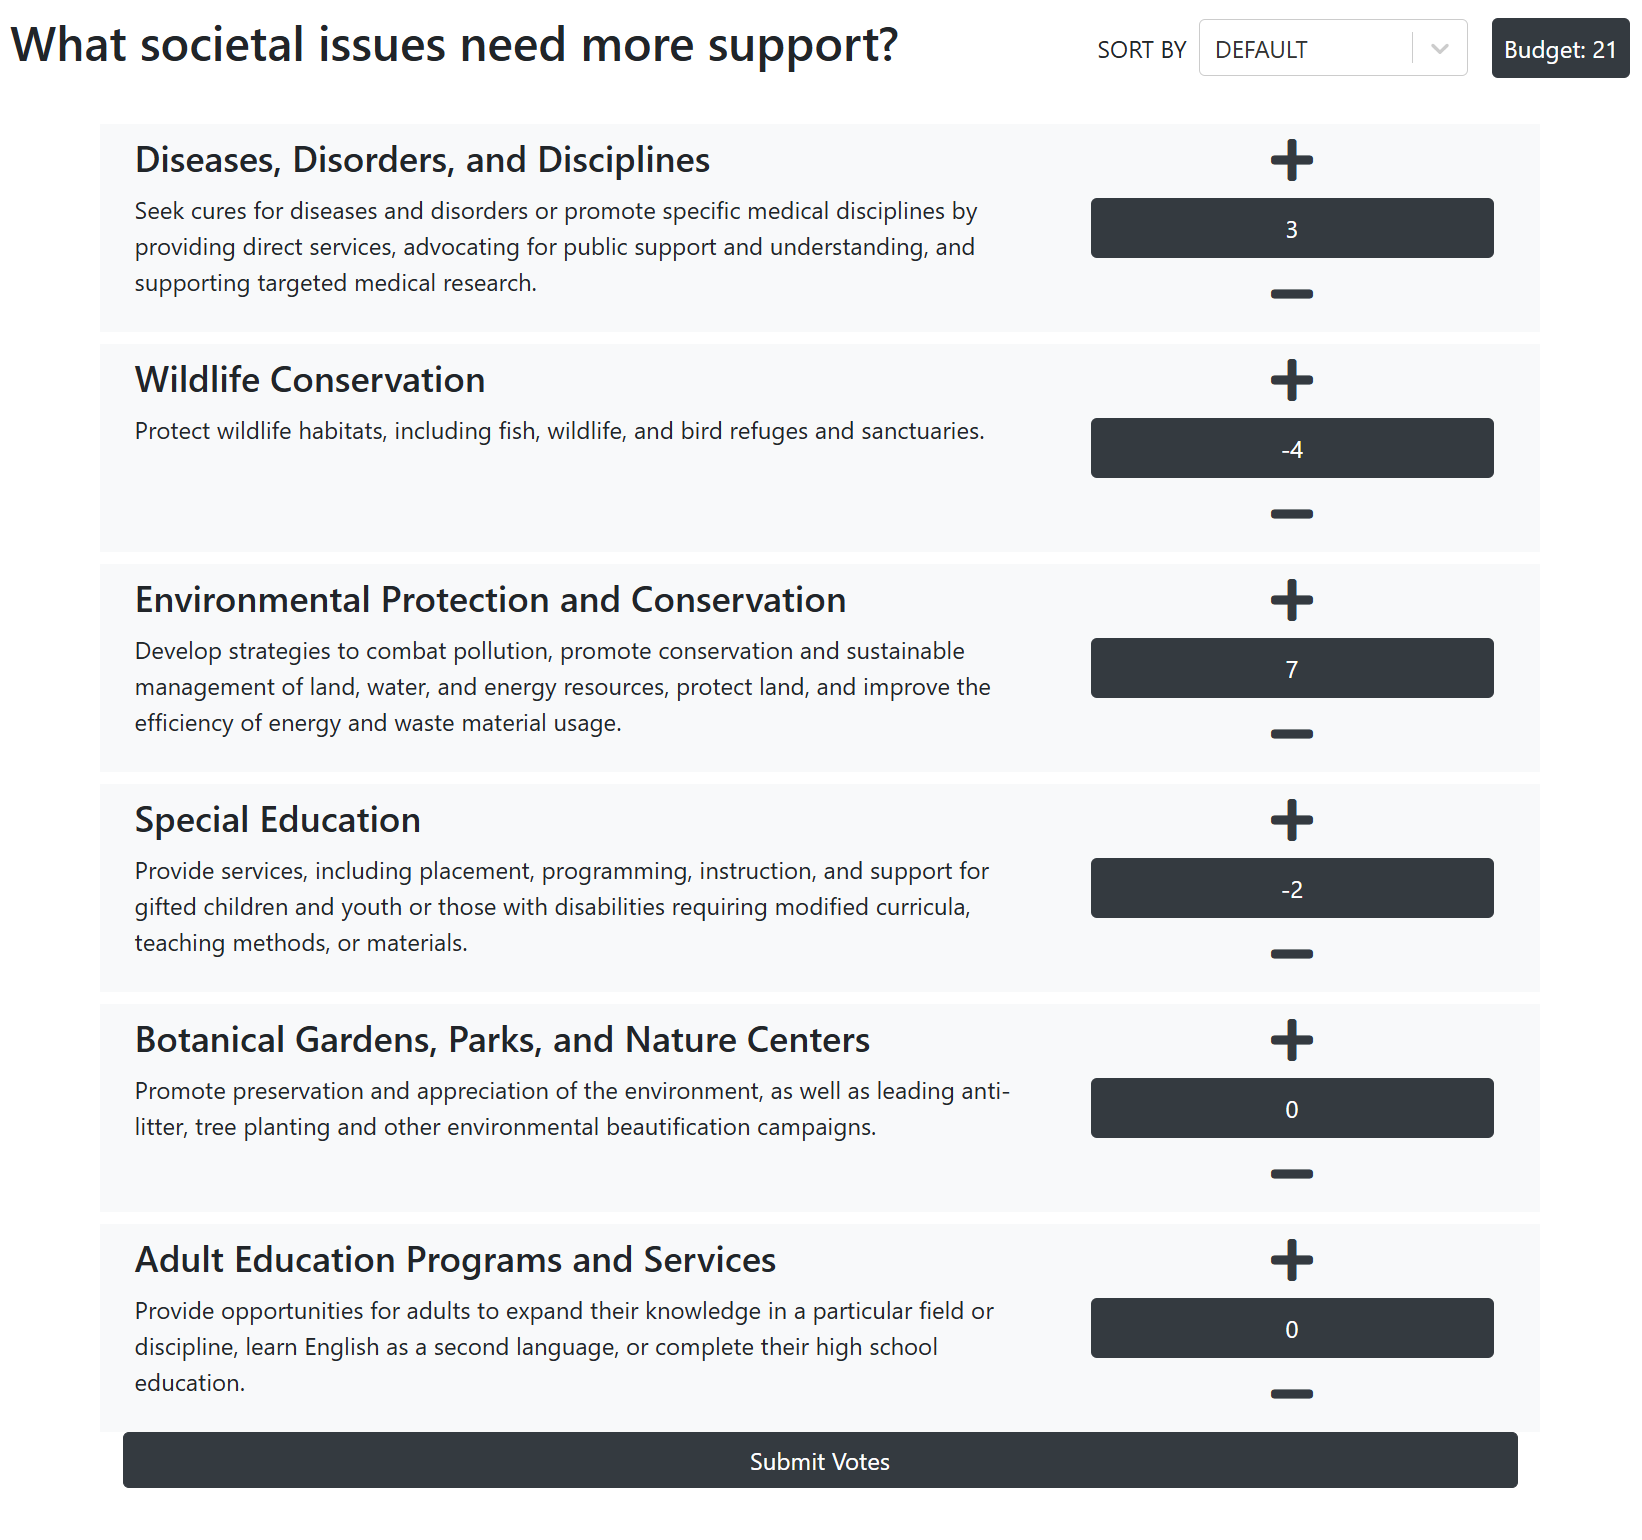
\includegraphics[width=\textwidth]{content/image/curr_interface/geek.sg_interface.png}
        \caption{An open-source QV interface~\cite{yehjxraymondYehjxraymondQvapp2024} with a publicly available service.}
        \label{fig:yehInterface}
    \end{subfigure}
    \hfill
    \begin{subfigure}[b]{0.3\textwidth}
        \centering
        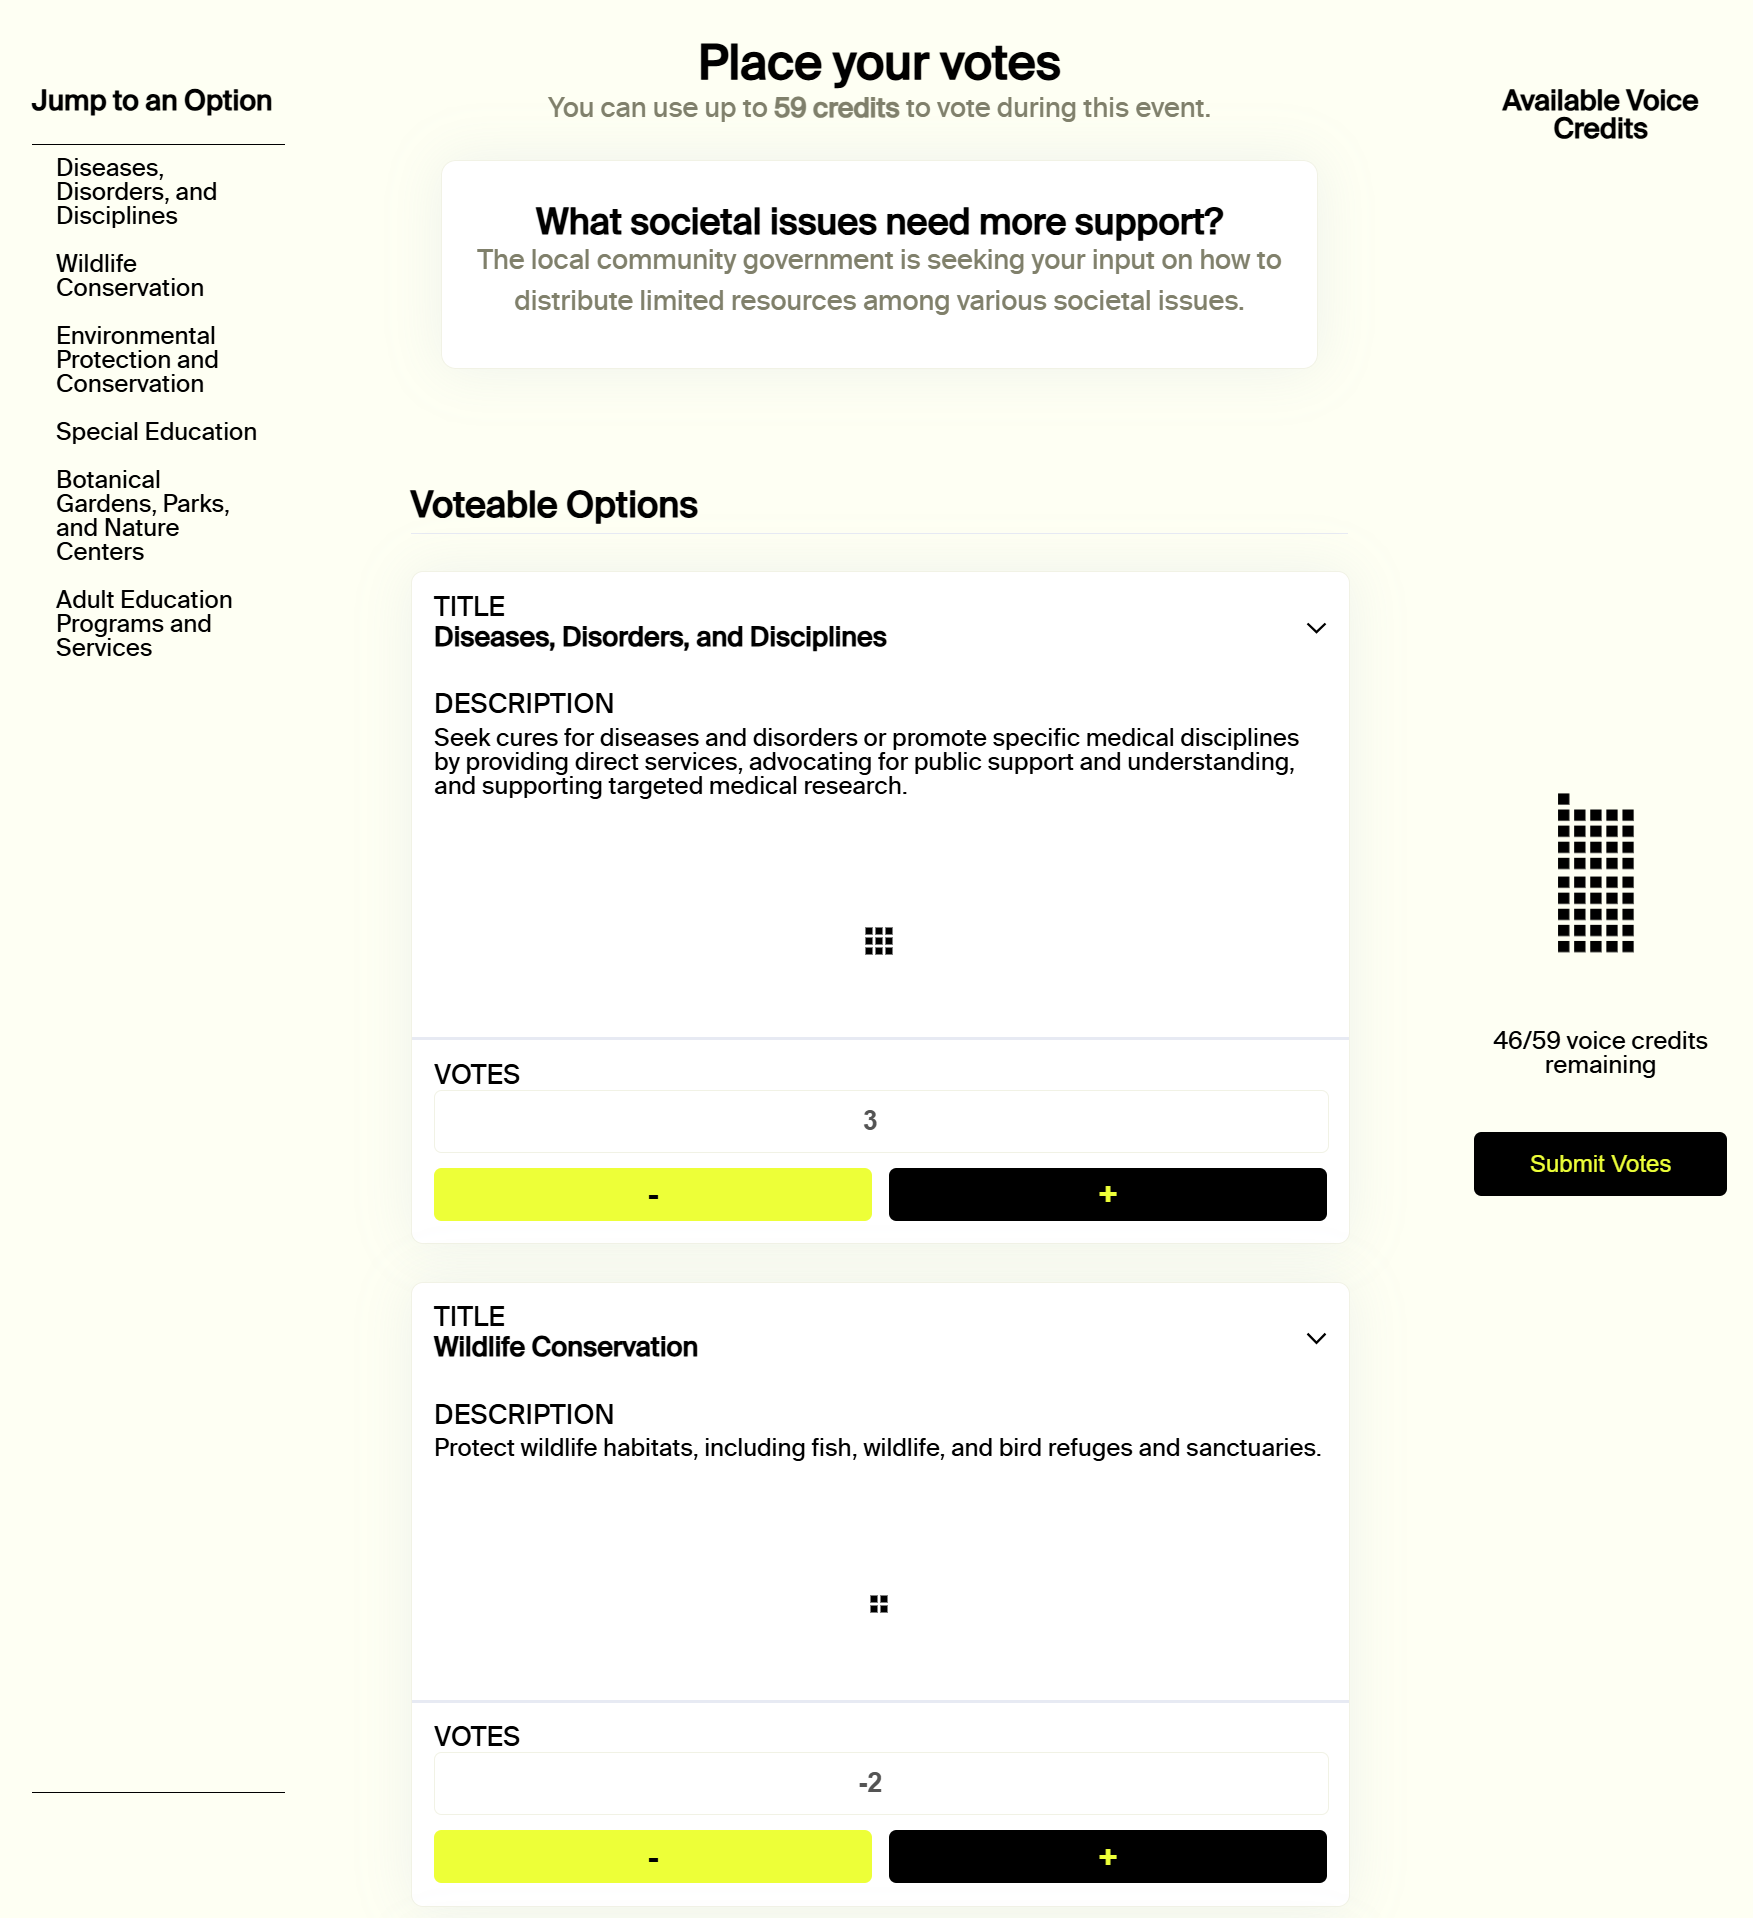
\includegraphics[width=\textwidth]{content/image/curr_interface/rxc_interface.png}
        \caption{An open-source QV interface~\cite{RadicalxChangeQuadraticvoting2024} forked from GitCoin~\cite{ReadWhitepaperGitcoin} used by the RadicalxChange community~\cite{RxC}.}
        \label{fig:rxcvotingInterface}
    \end{subfigure}
    \vskip\baselineskip
    \begin{subfigure}[b]{0.3\textwidth}
        \centering
        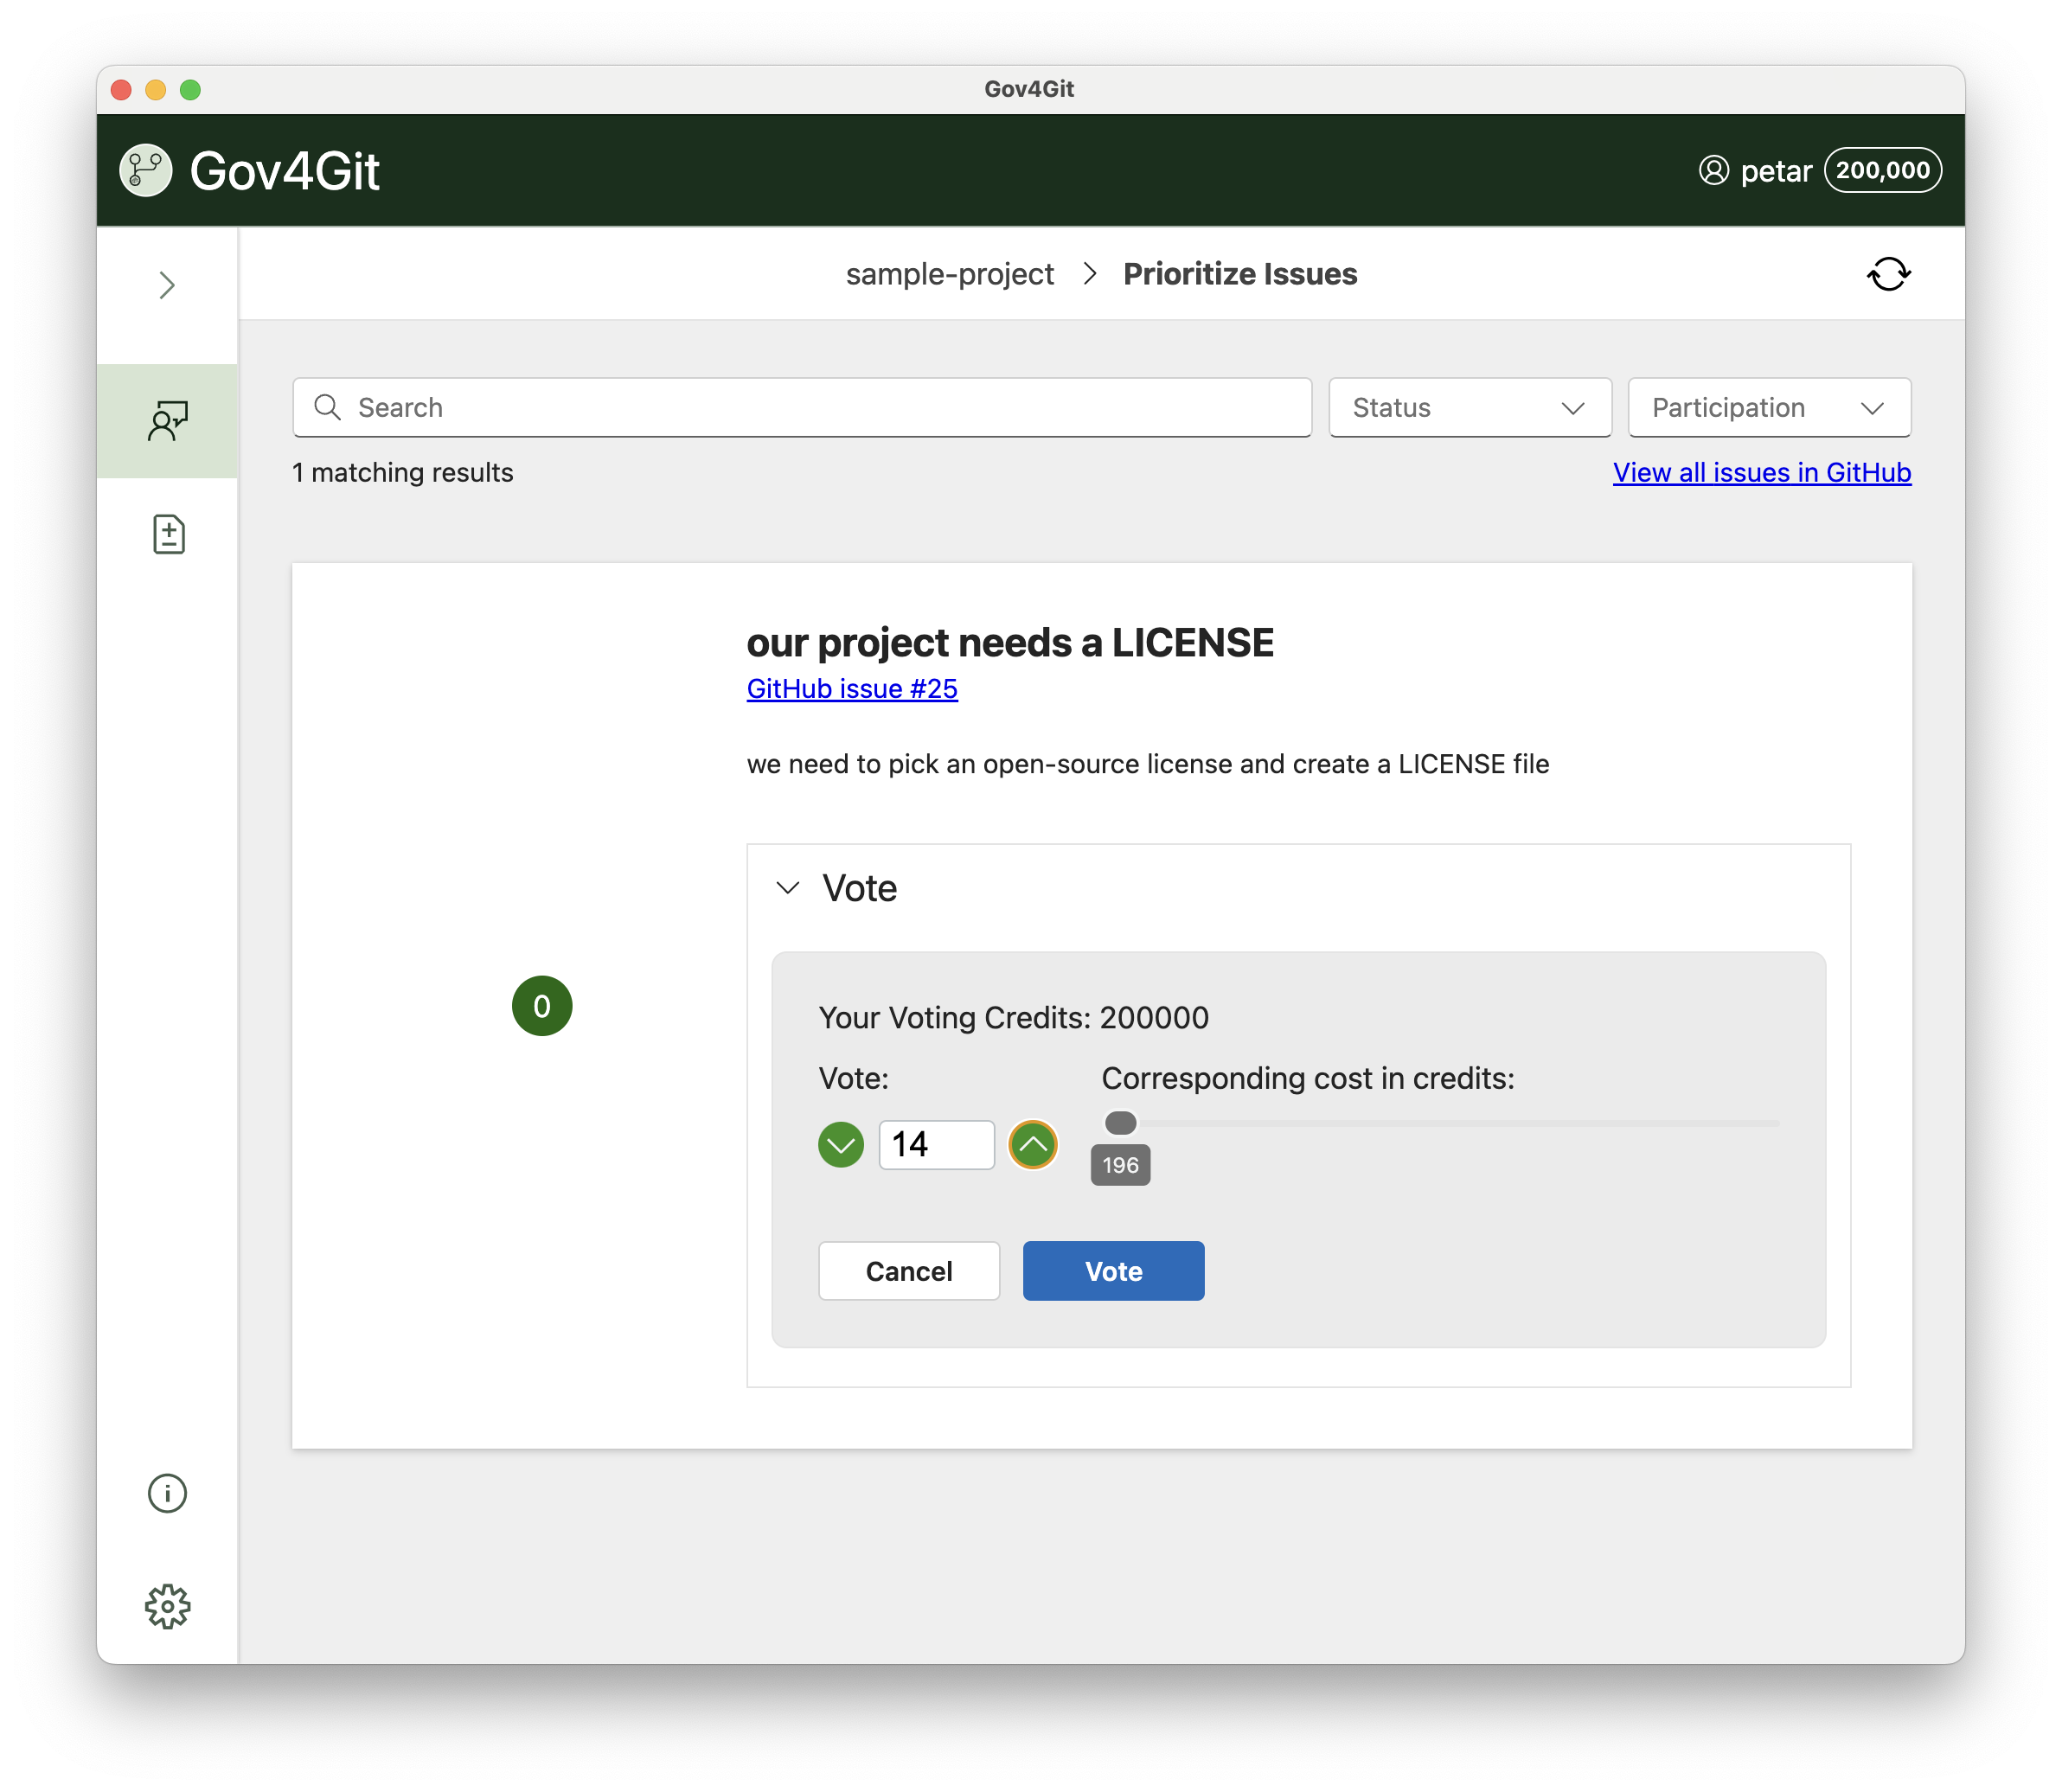
\includegraphics[width=\textwidth]{content/image/curr_interface/appvote.png}
        \caption{The interface designed for gov4git~\cite{Gov4gitDecentralizedPlatform2023}.}
        \label{fig:gov4gitInterface}
    \end{subfigure}
    \begin{subfigure}[b]{0.3\textwidth}
        \centering
        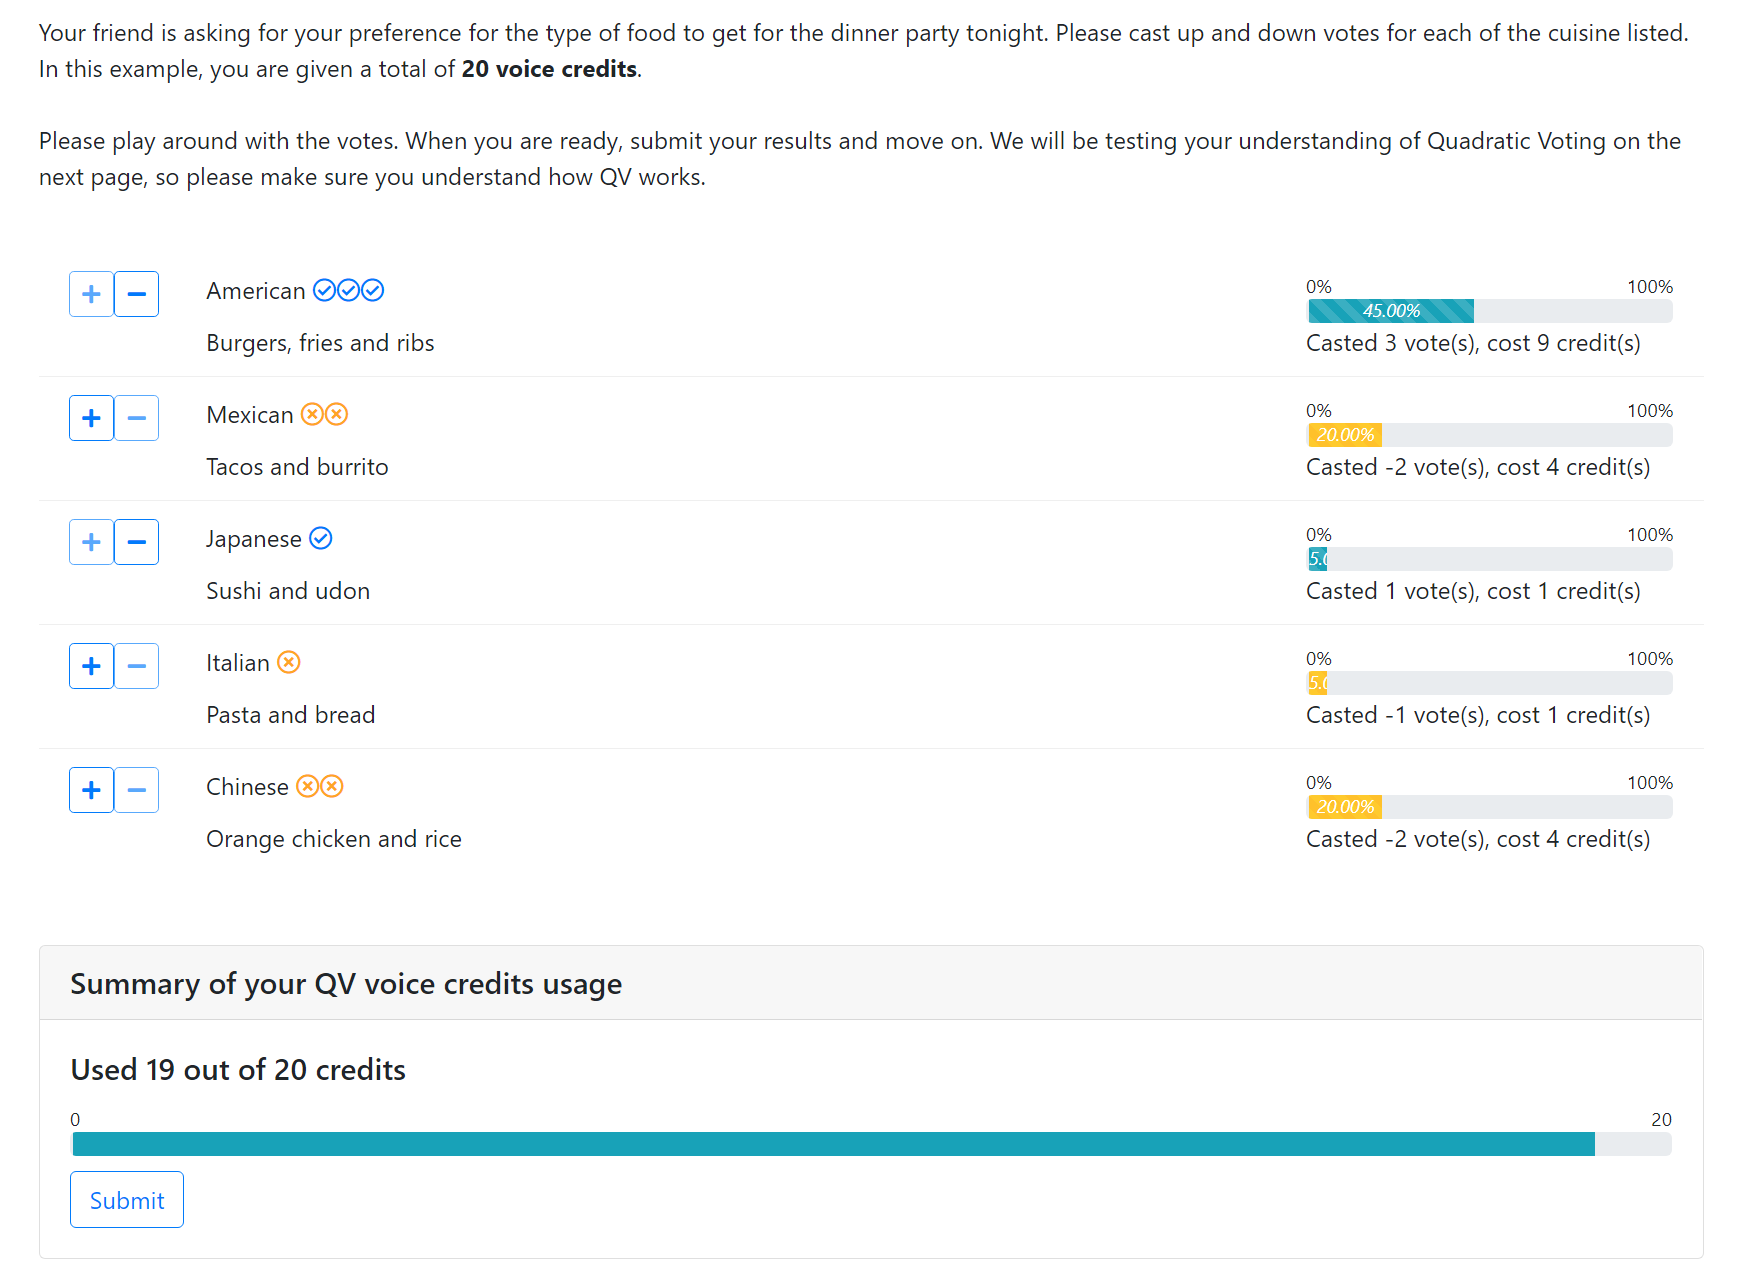
\includegraphics[width=\textwidth]{content/image/curr_interface/cheng_qv.png}
        \caption{The interface used in the research by~\textcite{chengCanShowWhat2021}.}
        \label{fig:chengInterface}
    \end{subfigure}
    \caption{Recent implementations of interfaces applying the quadratic mechanism.}
    \label{fig:qv_interface_external}
\end{figure}

\section{Interface Design}
\label{sec:interfaceDesign}
In this study, we developed an interactive interface for QS based on prior literature for the experiment condition. Since there are no studies and standard interfaces associated with quadratic survey-based tools, we designed to construct two versions of the interface to study how interactive components influenced participants' cognitive load and behaviors. In the following subsections, we describe and justify these interface design decisions.

\subsection{Text-based Interface}
First, we surveyed the current implementation of QV interfaces to understand the development of such tools. We present a selection in Figure~\ref{fig:qv_interface_external}. All five interfaces retain and present the following components:
\begin{itemize}
    \item Option list: A list of options contesting for votes.
    \item Vote Controls: Two buttons to increase and decrease votes associated for each option.
    \item Individual vote tally: A representation of votes associated with an option.
    \item Summary: A summary that automatically calculates the cost across options and the remaining budget.
\end{itemize}

We constructed a text-based interface that included all five components but removed the use of emojis (i.e., thumbs up and thumbs down present in Figure~\ref{fig:wedesignInterface}), progress bars, and other visualizations in the summary section (i.e., progress bars in Figure~\ref{fig:wedesignInterface} and~\ref{fig:chengInterface} or blocks presented in Figure~\ref{fig:rxcvotingInterface}), and the visual cues for individual vote counts (i.e., the colored counts and icons present in Figure~\ref{fig:gov4gitInterface} and~\ref{fig:chengInterface}).

Prior literature suggests that the use of emojis might influence the interpretations of surveys~\cite{herringGenderAgeInfluences2020} and decrease user satisfaction~\cite{toepoelSmileysStarsHearts2019}. Prior literature also noted that not all data visualization elements reduce cognitive demand~\cite{huangMeasuringEffectivenessGraph2009a}. Even though effective visaulization can aid decision making, it remains an open question that this study does not aim to address, thus we also removed all visualization elements such as blocks, progress bars, and percentage indicators. Last, different from all these interfaces, we decided to present all the options on the same screen. Prior research emphasizes the importance of placing all the options on the same digital ballot screen to avoid losing votes (missing citations). This echoes the proverb ``out of sight, out of mind,'' where individuals might be biased toward options that are shown to them and additional effort is required for individuals to retrieve specific information if options are hidden (citation needed).

These design decisions led to the interface shown in Figure~\ref{fig:textInterface}. The interface contains the question prompt at the top of the screen. The options are presented in the list underneath the prompt. Survey respondents can update the votes by selecting from a dropdown that provides all possible voting options and cost given the number of credits. A small summary box to the right of the interface shows the current total cost and the remaining credits for the respondent. Option options are always randomly presented on the interface to avoid ordering bias~\cite{ferberOrderBiasMail1952, couperWebSurveyDesign2001}.

\begin{figure}[H]
    \centering
    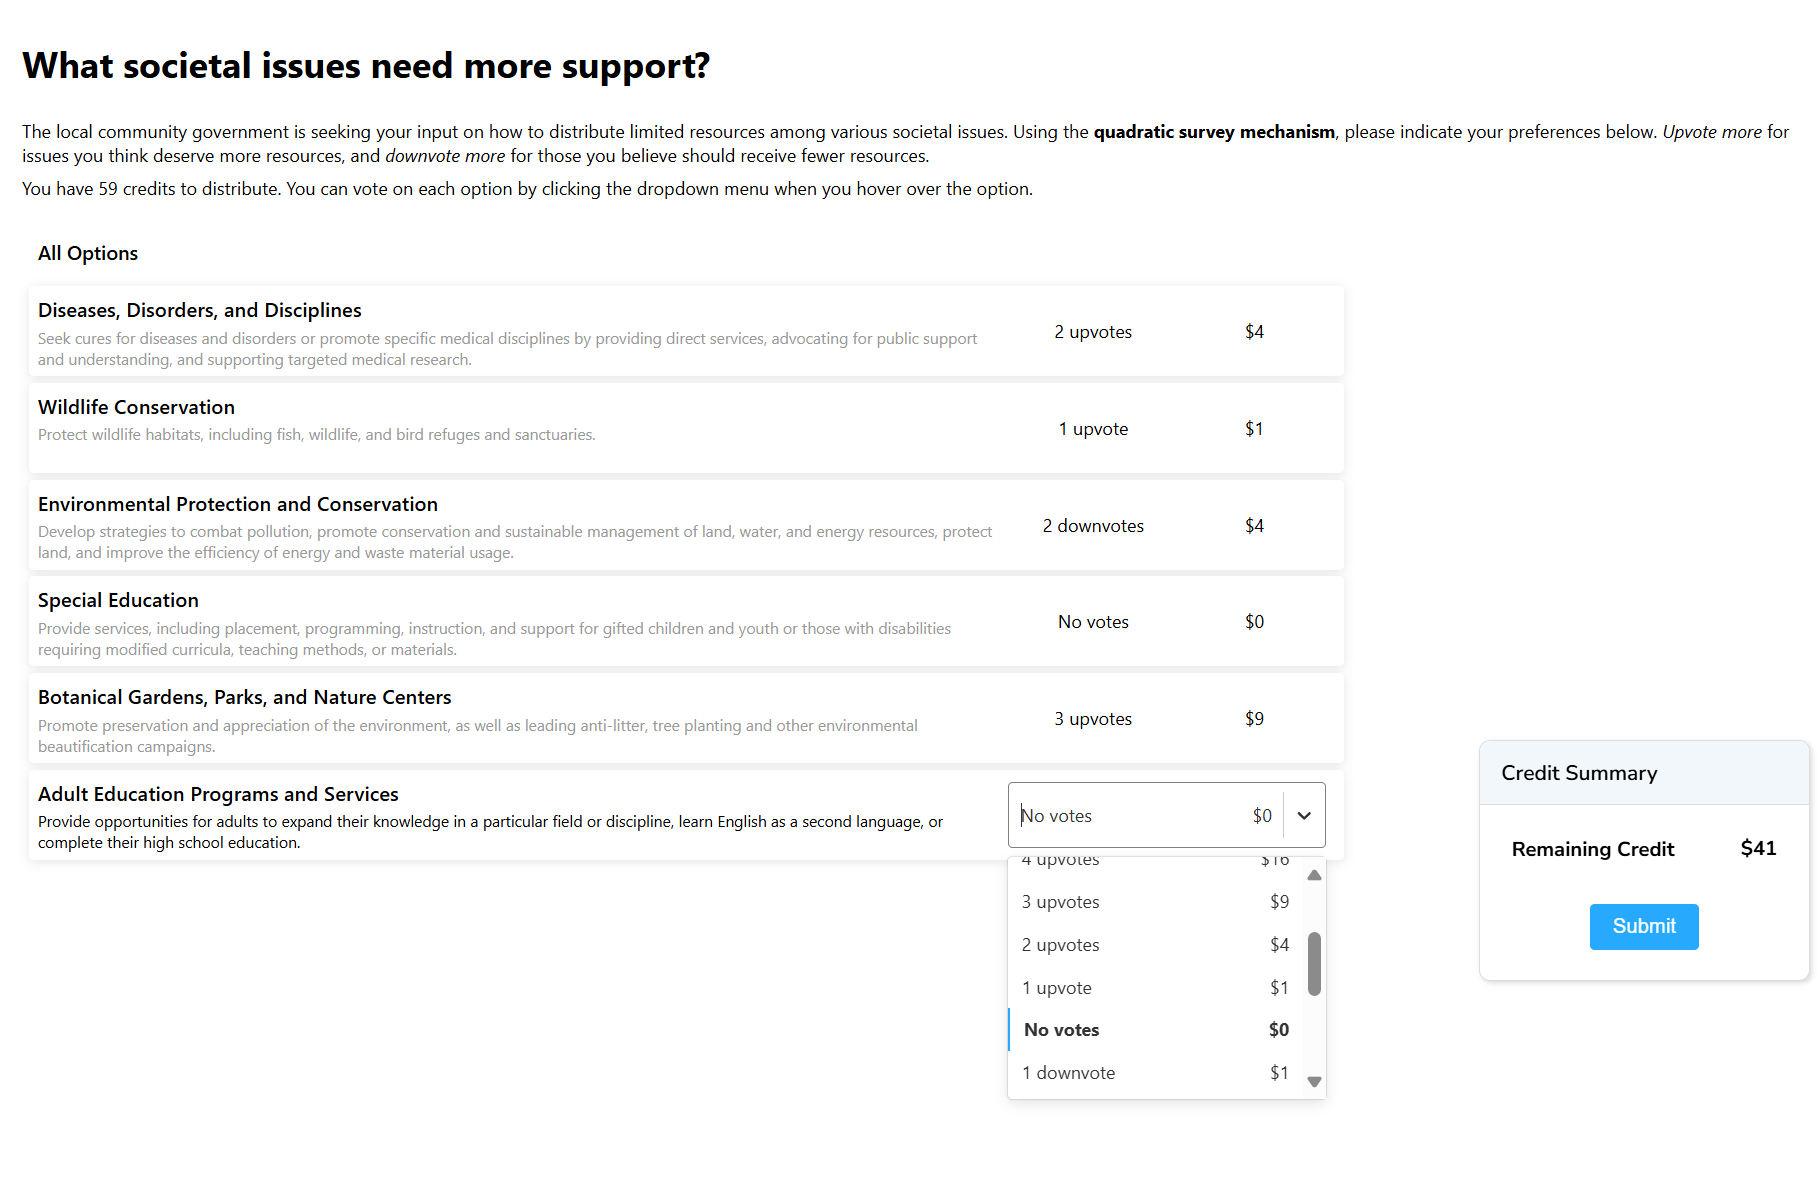
\includegraphics[width=0.6\textwidth]{content/image/text_interface.png}
    \caption{The text-based interface}
    \label{fig:textInterface}
\end{figure}

\subsection{Interactive Interface}
The design objective for the interactive interface is to facilitate preference construction and reduce cognitive load. The interactive interface, shown in Figure~\ref{fig:interactiveInterface}, builds additional interactive elements on top of the text interface to maintain consistency that allows comparison of the direct manipulation of the designed interactive elements. We designed two additional components: An additional organization step prior to voting and a drag-and-drop interface throughout the QS responding session informed through prior literature.

\paragraph{A two phase approach}

If preferences are constructed, by nature, they consist of a series of constructed decision-making processes~\cite{lichtensteinConstructionPreference2006}. Two major decision-making theories inform the design decision of a two-step interaction interface design:~\textcite{montgomeryDecisionRulesSearch1983}'s Search for a Dominance Structure Theory (Dominance Theory) and~\textcite{svensonDifferentiationConsolidationTheory1992}'s Differentiation and Consolidation Theory (Diff-Con Theory). The former suggests that decision-makers prioritize creating dominant choices to minimize cognitive effort by focusing on evidently superior options~\cite{montgomeryDecisionRulesSearch1983}. The latter describes a two-phase process where decisions are formed by initially ~\textit{differentiation} among alternatives and then~\textit{consolidating} these distinctions to form a stable preference~\cite{svensonDifferentiationConsolidationTheory1992}. Both theories guided the design decision in building the interactive experience to reduce initial decision dimensions and the mental procedures involved in emphasizing relatively important options and form decisions.

Hence, the two-phase design -- organize then vote -- aims to facilitate this cognitive journey explicitly. The first phase focuses on differentiating and identifying dominant options, enabling survey respondents to preliminarily categorize and prioritize their choices. The second phase presents these categorized options in a comparable manner, with drag-and drop functionality, enhancing one's ability to consolidate preferences. This structured approach aims to construct a clear decision-making procedure that reduces cognitive load and enhances clarity and confidence in the decisions made.

\paragraph{Phase 1: Organization Phase}
The goal of the organization phase is to support participants in identifying dominating options or partitioning options into differentiable groups. In this section, we first describe how the interaction works, then we detail reasons for the different design decisions implemented.

The organizing interface, depicted on the left side of Figure~\ref{fig:interactiveInterface}, sequentially presents each survey option. Participants select a response among three ordinal categories -- lean positive, lean negative, or lean neutral. Once selected, the system will move that option to the respective category. Participants can skip the option if they do not want to indicate a preference. Options within the groups are draggable and rearrangeable to other groups should the participants wish.

\textcite{strackThinkingJudgingCommunicating1987}'s research shows that upon understanding a survey question, respondents either recall a prior judgment or construct a new one when completing an attitude survey. In addition, revealing one option at a time gates the amount of information presented to the survey respondent and thereby reduces the extraneous load~\cite{swellerCognitiveLoadTheory2011}. This process allows participants to form or express opinions on individual options incrementally.

The three possible options, positive, neutral, and negative, aim to scaffold participants in constructing their own choice architecture~\cite{munscherReviewTaxonomyChoice2016, thalerNudgeImprovingDecisions2008a}, which strategically segments options into diverse and alternative choice presentations while avoiding the biases from defaults. We believe that these three categories are sufficient for participants to segment the options. However, we chose not to limit the number of options one can place into a category to prevent restricting user agency, a core user interface design principle~\cite{norman2013design}.

Immediate feedback displaying the placement of options and allows participants to rearrange them via drag-and-drop adheres to key interface design principles~\cite{norman2013design}. At the same time, it allows finer grain control for individuals to surface dominating options and creating differentiating groups of options.

This design underwent paper prototypes and various iterations, which all maintained the combination of these theoretical bases aimed at reducing cognitive load and scaffolding the decision-making process. We describe these iterations and the design process in Appendix A.
\begin{figure}[h]
    \centering
    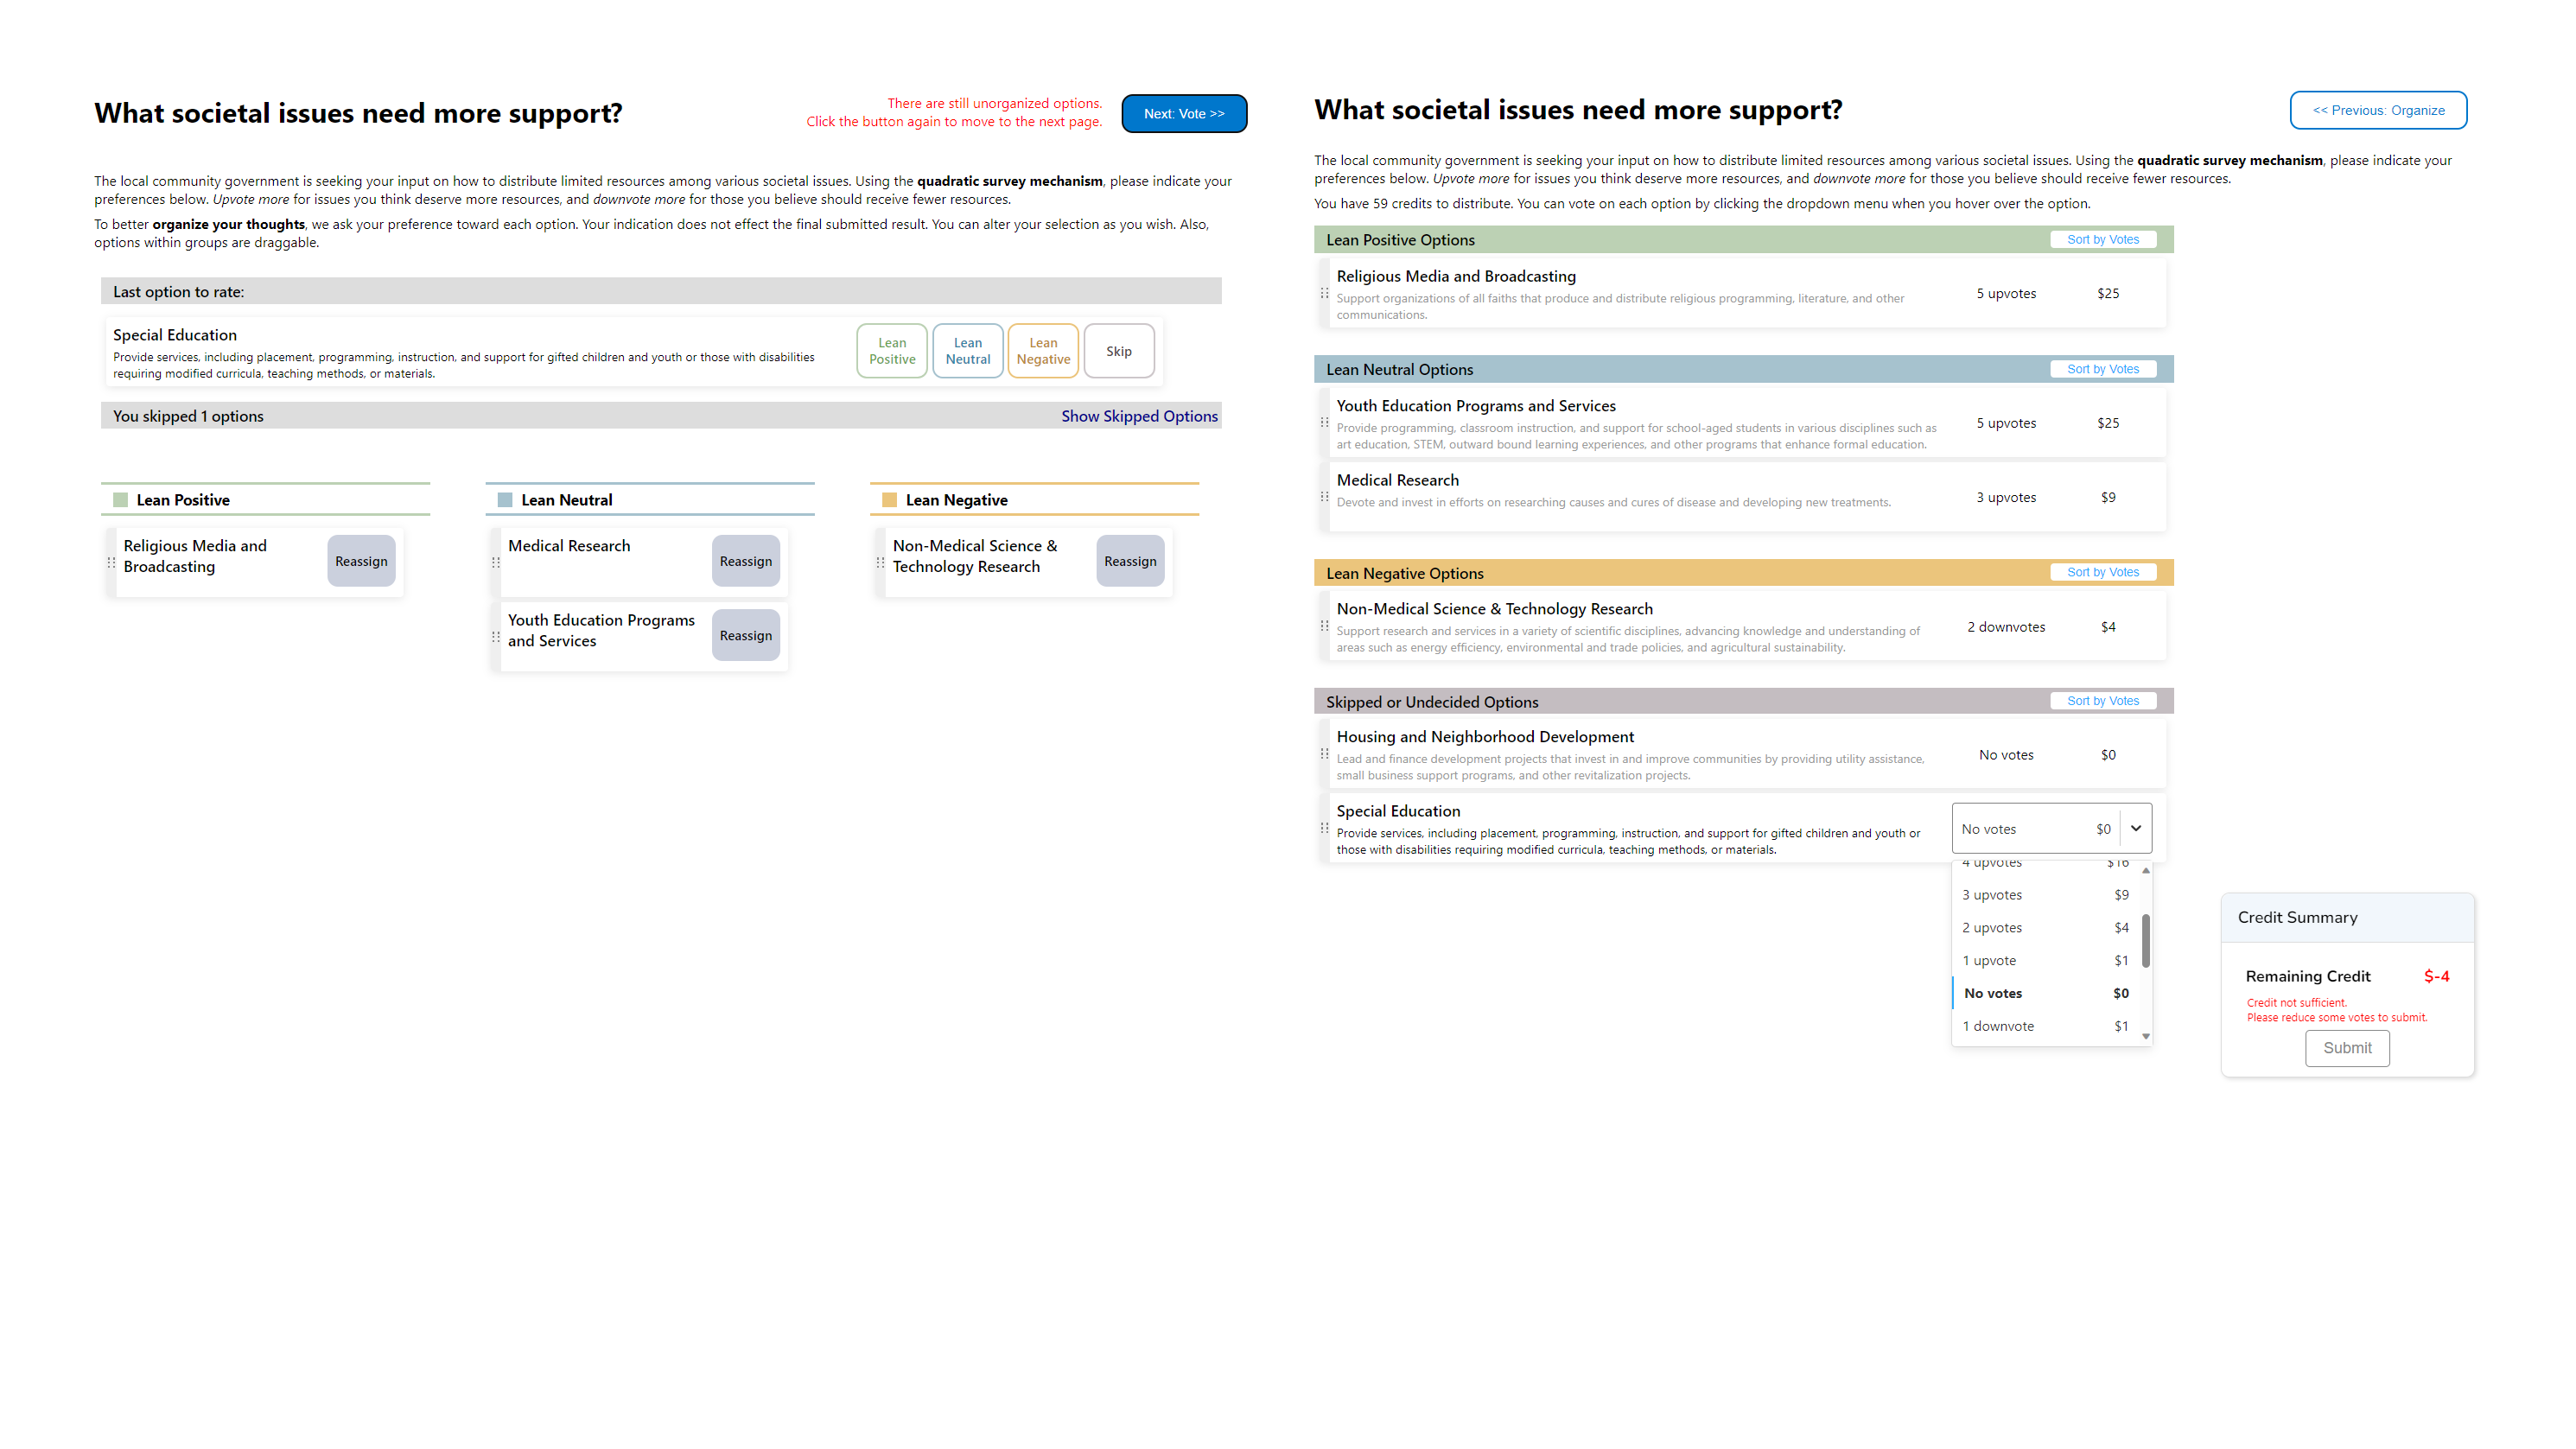
\includegraphics[width=1\textwidth]{content/image/interface.png}
    \caption{The interactive interface}
    \label{fig:interactiveInterface}
\end{figure}

\paragraph{Phase 2: Interactive Voting Phase}

The objective of the voting phase is to facilitate the consolidation of differentiated options through interactive elements while reinforcing the differentiation across options constructed by participants from the previous phase. This facilitation is achieved by retaining the drag-and-drop functionality for direct manipulation of position and enabling sorting within each category.

Options are displayed as they were categorized within each category from the previous step and in the following section orders -- lean positive, lean neutral, lean negative, and skipped or undecided as detailed on the right-hand side of Figure~\ref{fig:interactiveInterface}. The Skipped or Undecided category contains options left in the organization queue, possibly because survey respondents have a pre-existing preference or choose not to organize their thoughts further. The original order within these categories is preserved to maintain and reinforce the differentiated options. Respondents have the flexibility to return to the organization interface at any point during the survey to revise their choices.

In the interactive interface, options remains draggable, enabling participants to modify or reinforce their preference decisions as needed. Each category features a sort-by-vote function that enables reordering within the same category. Although these interactions do not influence the final voting outcome, they are designed to support consolidation and positional proximity in information organization.This design aims to automate the grouping of similar options while providing an intuitive drag-and-drop mechanism, thereby facilitating decision-making by placing similar options near each other. This echoes the principles of the proximity compatibility principle, particularly emphasizing spatial proximity and mental compatibility~\cite{wickens1990proximity}. The interface design anticipates that participants will find it easier to consolidate their choices when similar options are positioned close together, thereby reducing cognitive load.

While multiple interaction mechanisms exist, drag-and-drop has been extensively explored in rank-based surveys. For instance,~\textcite{krosnick2018measurement} demonstrated that replacing drag-and-drop with traditional number-filling rank-based questions improved participants' satisfaction with little trade-off in their time. Similarly,~\textcite{timbrook2013comparison} found that integrating drag-and-drop into the ranking process, despite potentially reducing outcome stability, was justified by the increased satisfaction and ease of use reported by respondents. The trade-off is deemed worthwhile as QS does not use the final position of options as part of the outcome if it significantly enhances user satisfaction and usability~\cite{rintoulVisualAnimatedResponse}.
Together, these design decisions lead to our belief that a two-step interactive interface with direct interface manipulation can reduce the cognitive load for survey respondents to form preference decisions when completing QS.

